\documentclass{scrartcl}
\usepackage{color}
\usepackage{graphicx}
\usepackage{float}
\setkomafont{disposition}{\bfseries}

\begin{document}

%Title, Author, Experiment, Date	
\title { {ECE385} \\
		{\large \normalfont Spring 2016} \\
		{\large \normalfont Experiment \#1 } \\
		\vspace{60mm}
		{\large \normalfont 2-to-1 Multiplexer TTL Circuit} \\
		\vspace{60mm}
		{\large \normalfont Eric Meyers} \\
		{\large \normalfont Section ABG} 
		\vfill
	}

	
\clearpage
\maketitle
\thispagestyle{empty}
\newpage

%SECTION 1 - Introduction
\section{Introduction}
The purpose of this lab is to demonstrate the impact of using a glitch-free 2-to-1 multiplexer using Transistor-Transistor Logic (TTL) chips on a protoboard. This experiment consisted of two parts: (1) Designing and constructing a glitch-prone 2-to-1 multiplexer, connecting a 1 MHz square-wave input to the select-line, and analyzing its output waveform and (2) designing and constructing a glitch-free 2-to-1 multiplexer, connecting a 1 MHz square-wave input to the select-line, and analyzing its output waveform. Static hazards were also explored during this lab and are explained when necessary below.  

 %SECTION 2 - Description of Circuits
 \section{Description of Circuits}
As stated in the introduction, there are two circuits created in this experiment. The first one being a glitch-prone 2-to-1 multiplexer and the second being a glitch-free 2-to-1 mulitplexer. Both Part A and Part B are explained in detail below. \\

Part A: The glitch-prone 2-to-1 multiplexer was constructed using one SN7400 Quad 2-Input NAND chip. In the pre-lab, a 2-to-1 multiplexer was designed by first creating a Karnaugh-Map (shown below in Figure 1), then selecting the optimal minterms and constructing an AND-OR circuit (Z =  (A$\land$B) $\lor$ ($\neg$B$\land$C)). This was then converted to a NAND-NAND circuit using deMorgan's Laws, and constructed on a protoboard. \\\\Power was then connected to the protoboard and the A and C input were driven to high, while a 1 MHz square-wave was connected to the select line (B). The reason a square-wave was connected to the select-line was in order to test the reliability of the output and to, specifically, check for a glitch occuring on the falling edge of the input. 

\begin{figure} [H]
	\centering
	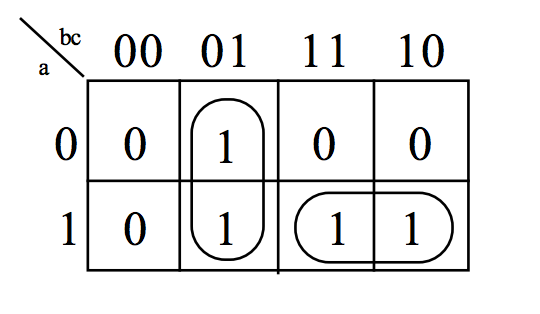
\includegraphics[scale = 0.5]{K-Map-Glitch-Prone.png}
	\caption{Glitch-Prone K-Map for Part A}
	\label{fig:k-map-glitch-prone}
\end{figure}


Part B: The glitch-free 2-to-1 multiplexer was constructed using two SN7400 Quad 2-Input NAND chips. The pre-lab adequately described the process for creating a glitch-free circuit by constructing the Karnaugh-Map first (shown below in Figure 2), selecting the optimal-minterms, then including a redundant minterm to avoid glitching. The redundant minterm is A $\land$ C. This brings our function to Z =  (A$\land$B) $\lor$ ($\neg$B$\land$C) $\lor$  (A$\land$C). The reason this additional minterm was added in was to ensure redundancy and to allow the circuit to operate glitch-free. \\

An identical procedure to Part A was performed on Part B, and a 1MHz square-wave was connected to the select-line (B), while the A and C lines were driven to high. 

\begin{figure} [H]
	\centering
	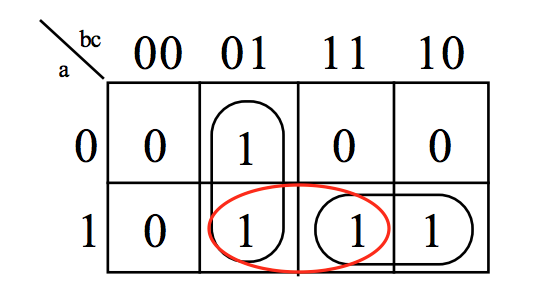
\includegraphics[scale = 0.5]{K-Map-Glitch-Free.png}
	\caption{Glitch-Free K-Map for Part B}
	\label{fig:k-map-glitch-free}
\end{figure}

%SECTION 3 - Component Layout Sheet
\section{Component Layout Sheet}
	%Component Layout Assignment and I/O
	\begin{figure} [H]
		\centering
		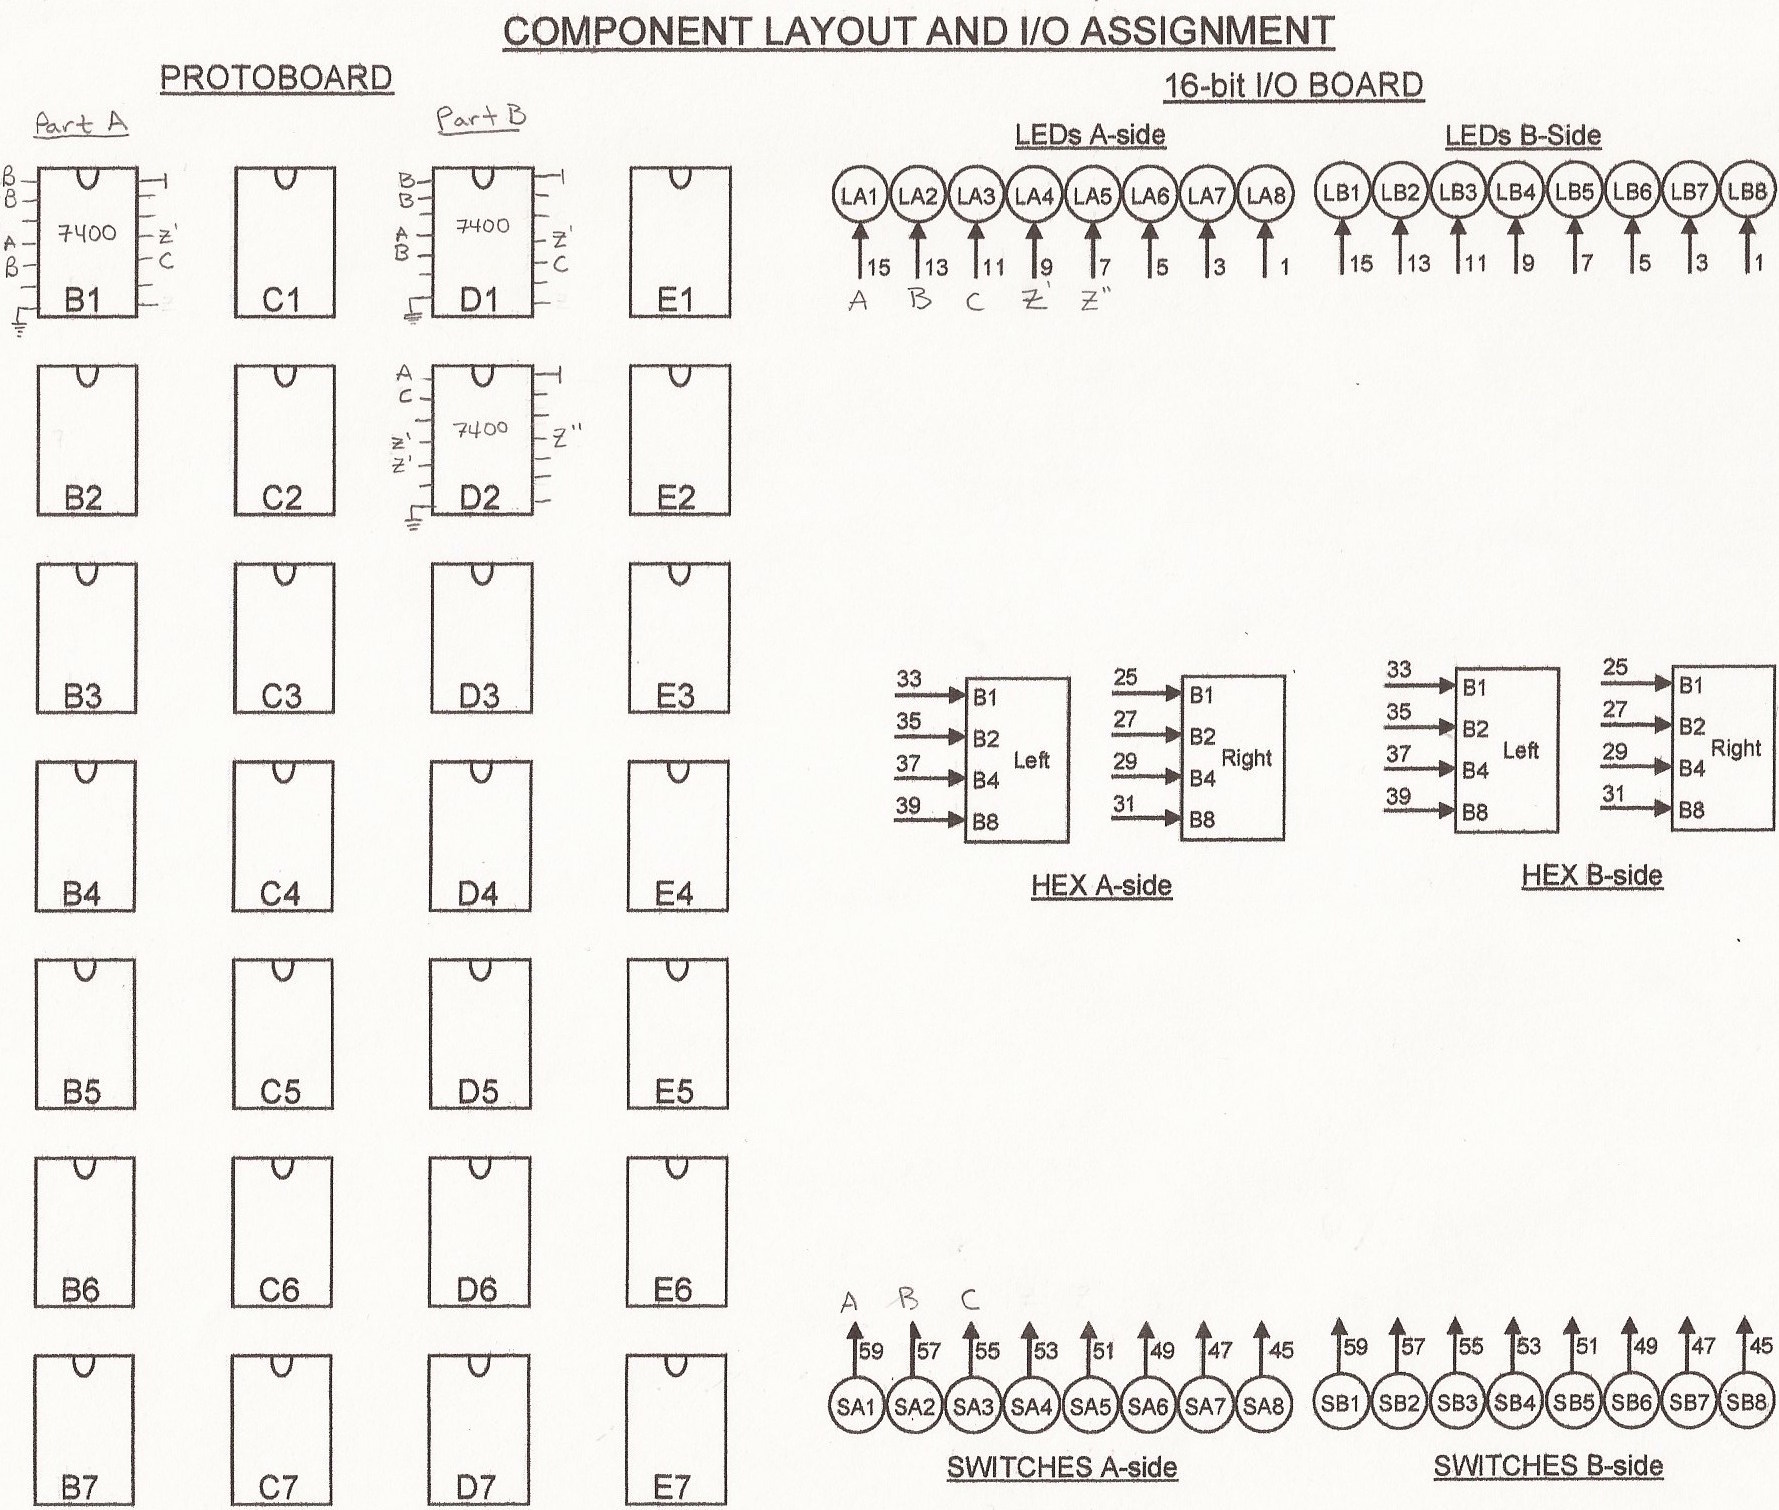
\includegraphics[scale = 0.2]{Layout_Diagram.jpeg}
		\caption{Component Layout Assignment and I/O Diagram}
		\label{fig:layout-diagram}
	\end{figure}

%SECTION 4 - Logic Diagrams
\section{Logic Diagrams}
	%Glitch-Prone Circuit Diagram
	\begin{figure} [H]
		\centering
		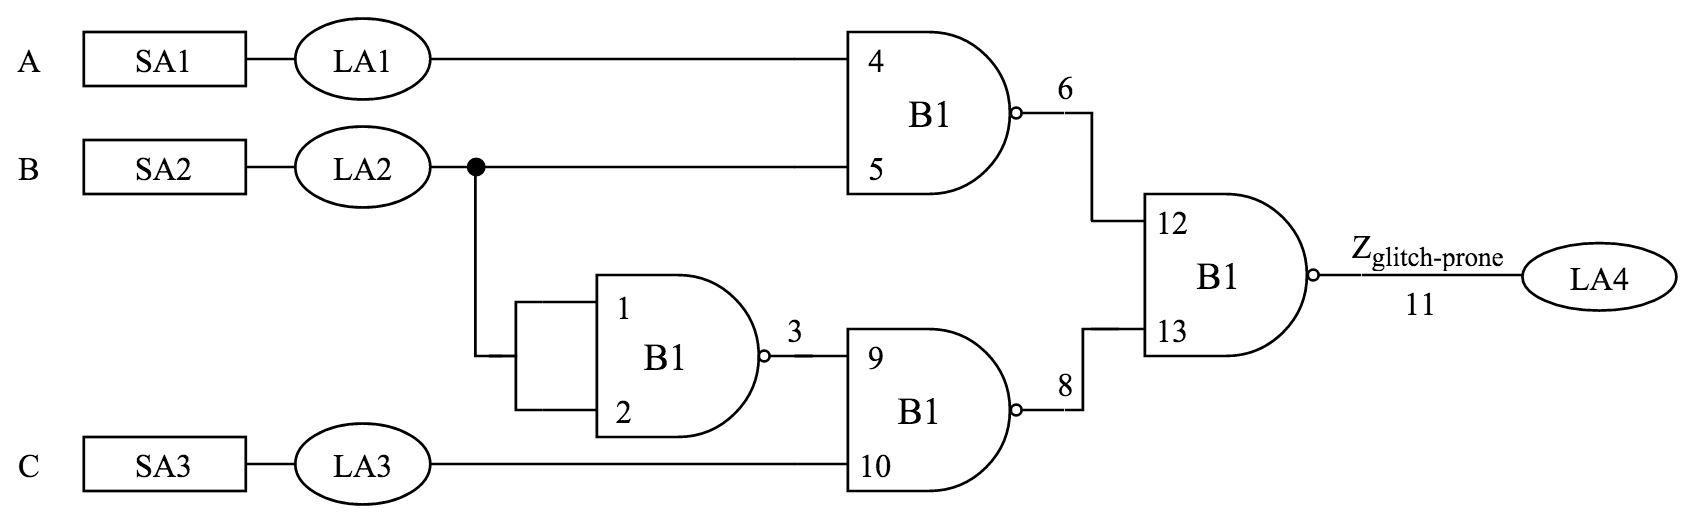
\includegraphics[scale = 0.5]{Glitch-Prone.png}
		\caption{Glitch-Prone Logic Circuit}
		\label{fig:glitch-prone}
	\end{figure}
	
	%Glitch-Free Circuit Diagram
	\begin{figure} [H]
		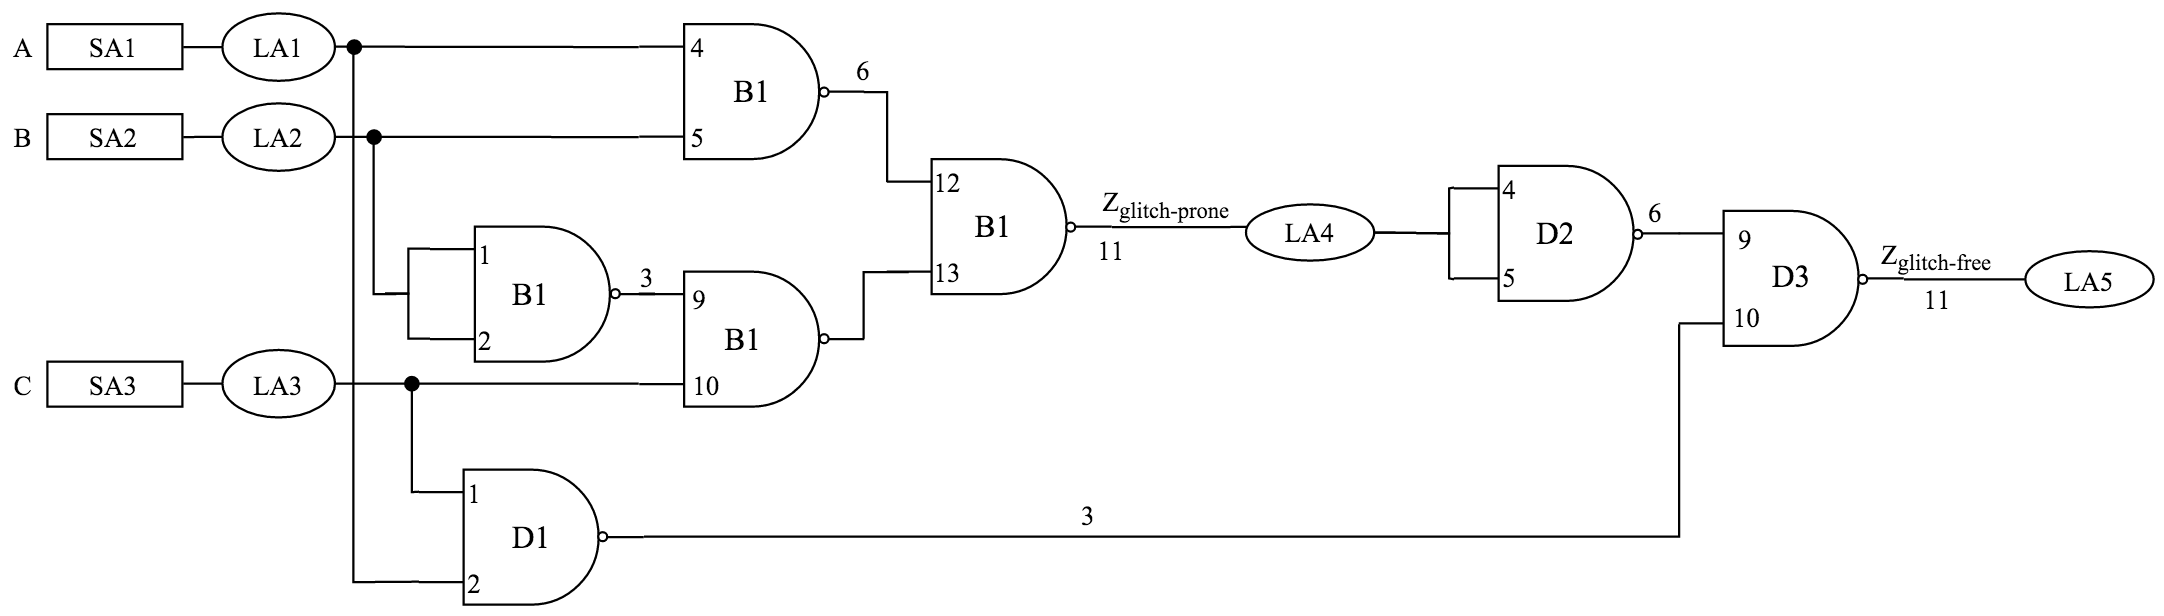
\includegraphics[width=\linewidth]{Glitch-Free-Circuit.png}
		\caption{Glitch-Free Logic Circuit}
		\label{fig:glitch-free}
	\end{figure}

%SECTION 5 - Experiment Documentation and Results
\section{Experiment Documentation and Results}
The results of the experiment are documented below. The first two tables (Table 1 and Table 2) are truth-tables summarizing the outputs of the constructed circuits in both part A and part B. The remaining two figures (Figure 6 and Figure 7) are readings generated from the oscilloscope of the respective circuits. 
	%Glitch-Prone Truth Table (Part A)
	\begin{table}[H]
		\centering
		\begin{tabular}{lll|l}
			A & B & C & Z \\ \hline
			0 & 0 & 0 & 0 \\
			0 & 0 & 1 & 1 \\
			0 & 1 & 0 & 0 \\
			0 & 1 & 1 & 0 \\
			1 & 0 & 0 & 0 \\
			1 & 0 & 1 & 1 \\
			1 & 1 & 0 & 1 \\
			1 & 1 & 1 & 1
		\end{tabular}
		\caption{Truth Table for Glitch-Prone Circuit (Part A)}
		\label{glitch-prone-truth-table}
	\end{table}

	%Glitch-Free Truth Table (Part B)
	\begin{table}[H]
		\centering
		\begin{tabular}{lll|l}
			A & B & C & Z \\ \hline
			0 & 0 & 0 & 0 \\
			0 & 0 & 1 & 1 \\
			0 & 1 & 0 & 0 \\
			0 & 1 & 1 & 0 \\
			1 & 0 & 0 & 0 \\
			1 & 0 & 1 & 1 \\
			1 & 1 & 0 & 1 \\
			1 & 1 & 1 & 1
		\end{tabular}
		\caption{Truth Table for Glitch-Free Circuit (Part B)}
		\label{glitch-free-truth-table}
	\end{table}

The first figure shows a static-1 hazard occuring at the falling edge of the 1 MHz square wave. A static-1 hazard is when the signal jumps/glitches down to a logic-0, when the actual output should instead be a logic-1. 

	%Glitch-Prone Oscilloscope Picture
	\begin{figure} [H]
		\centering
		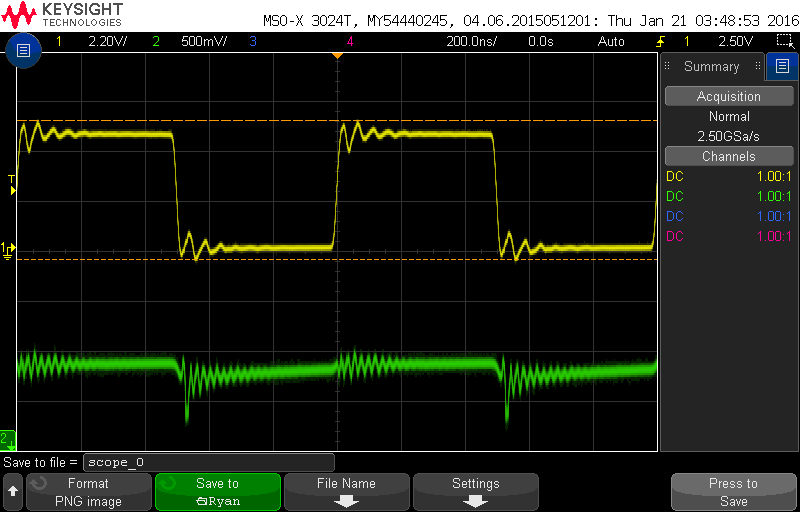
\includegraphics[scale = 0.35]{scope_0.png}
		\caption{Glitch-Prone Oscilloscope Reading for Part A}
		\label{fig:glitch-prone-oscilloscope}
	\end{figure}

	%Glitch-Free Oscilloscope Picture
	\begin{figure} [H]
		\centering
		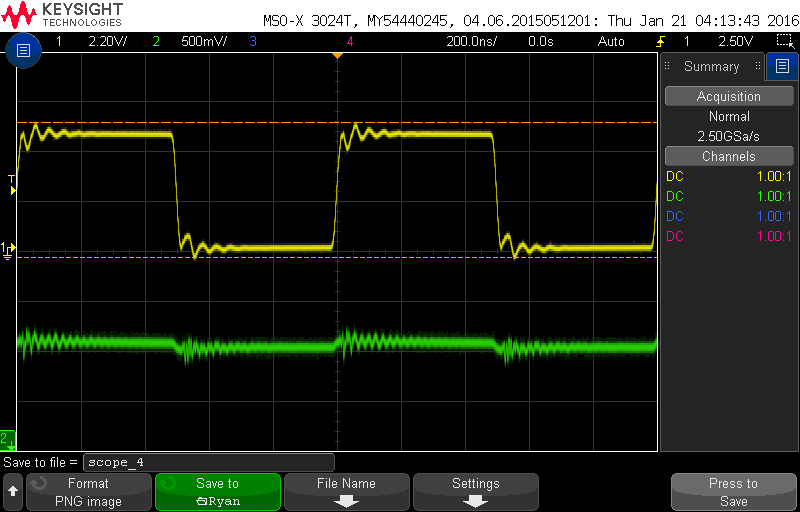
\includegraphics[scale = 0.35]{scope_4.png}
		\caption{Glitch-Free Oscilloscope Reading for Part B}
		\label{fig:glitch-free-oscilloscope}
	\end{figure}

%SECTION 6 - Post Lab Responses
\section{Post-Lab Responses}
1.) Given that the guaranteed \underline{minimum} propogation delay of a 7400 is 0ns and that its guaranteed \underline{maximum} delay time is 20ns, complete the timing diagram below for the circuit of part A.
	%Timing Diagram for Part-A
	\begin{figure} [H]
		\centering
		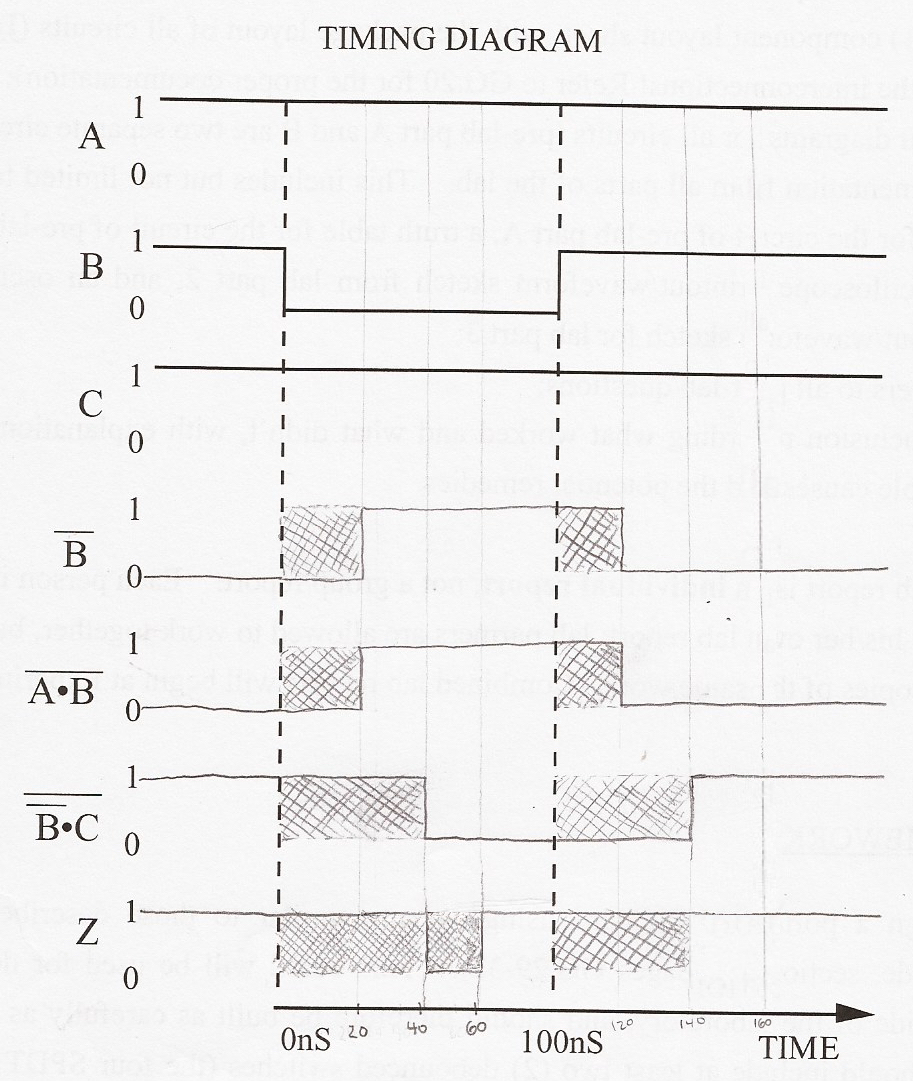
\includegraphics[scale = 0.4]{Timing_Diagram.jpeg}
		\caption{Timing Diagram for Part-A}
		\label{fig:timing-diagram}
	\end{figure}
	
\begin{itemize}
	\item How long does it take for the output Z to stabalize on the falling edge of B (in ns)? \\ \\
			It take approximately a maximum of 60 ns for the output Z to stabalize on the falling edge of B.
	\item  How long does it take on the rising edge (in ns)? \\ \\
			The output, Z, takes approximately a maximum of 40 ns to stabalize.
	\item Are there any potential glitches in the output, Z? If so, explain what makes these glitches occur? \\ \\
			Yes. There are potential glitch (a static-1 hazard) on the falling edge of the input B, as it is transitioning from 1 to 0. This is due to the fact that the propogation delay time for the A \& B is quicker than the propogation delay time for \~B \& C. This is known as a race-condition.
\end{itemize}
2.) Explain how and why the debouncer circuit given in General Guide Figure 17 (GG.32) works. Specifically, what makes it behave like a switch and how the ill effect of a mechanical contact bounces are eliminated? \\ \\
	The debouncer circuit is an S-R Latch with pull-down resistors of 5k$\Omega$. The S-R Latch has the special property that if either A = 1 or B = 1, it holds the stable state of either one. So, for example, if both A is 1 and B is 0, or vice-versa (which occurs when the switch is bouncing), the S-R NAND Latch holds the state of the previously contacted switch (so if the switch was previously at A (A = 1, B = 0), then it would hold the state of A=1 and B=0 - the same for the opposite case). This is because the output on the top NAND gate is fedback into the input of the bottom NAND gate and the same is done for the bottom NAND gate. 	
%SECTION 7 - Conclusion
\section{Conclusion}
As stated previously, both glitch-prone and a glitch-free 2-to-1 multiplexer TTL circuits were constructed in this lab. The circuit constructed in part A was prone to glitches (specifically a static-1 hazard) during the transition from 1 to 0 (on the falling edge) and this is shown in Figure 6 (the oscilloscope output). This is due to the propogation delay on TTL chips and depending on the number of NAND gates the signal must pass through to reach the output. These race-conditions must be eliminated at all costs due to their potential risks on a system. \\ \\ Another interesting experiment to perform would be to analyze the propogation delay and glitches using different chips and complex circuit arrangements. However, overall, for the purposes of this lab, many properties can be understood about TTL circuits and static hazards.
\end{document}    
